

\subsection{Fast Interaction Trigger (FIT)}

\begin{figure}[htbp]
\begin{center}
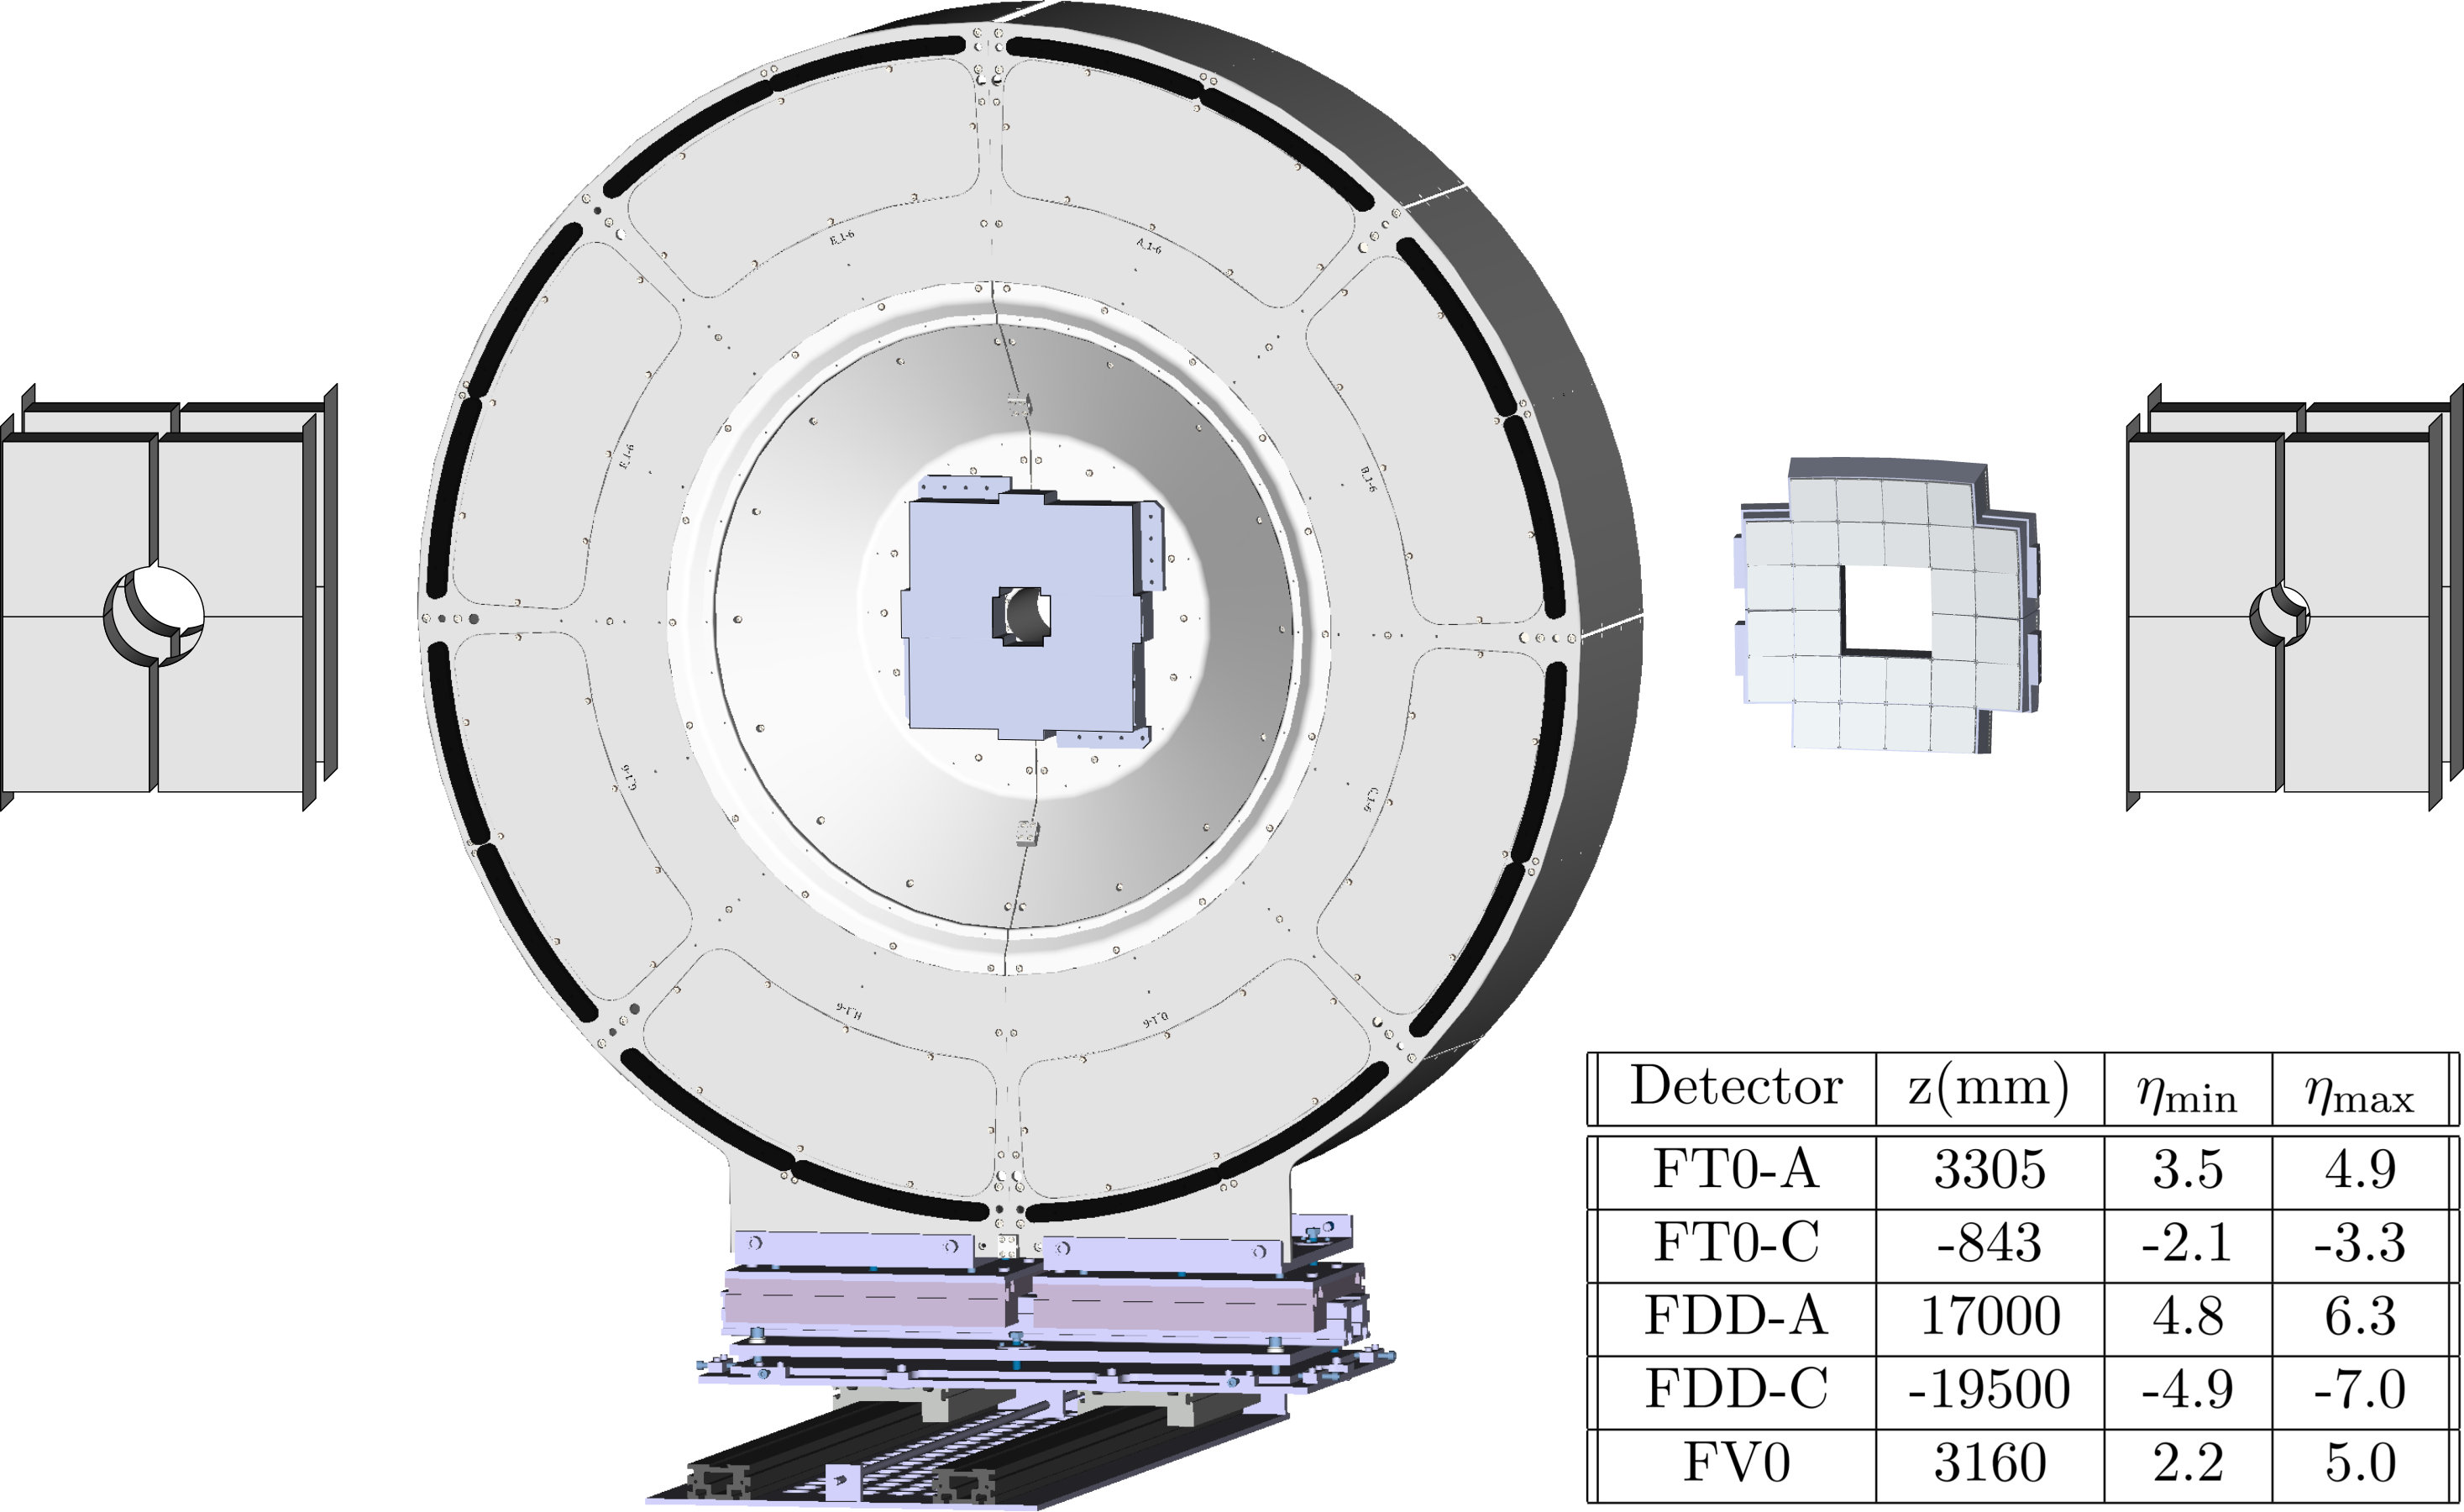
\includegraphics[width=0.8\linewidth]{fit/f40Fit3dCompleteTable.png}
\caption{View of FIT detectors illustrating the relative sizes of each component.  From left, FDD-A, FT0-A, FV0, FT0-C, FDD-C.  Note that FT0-A and FV0 have a common mechanical support. FT0-A is the small quadrangular structure in the centre of the large, circular FV0 support. Note that all are planar with the exception of FT0-C which has a concave shape centered on the IP.  The inset table lists the distance from the IP and the pseudorapidity coverage for each component.  }
\label{FITschematic}
\end{center}
\end{figure}

The Fast Interaction Trigger (FIT)\cite{Trzaska:2017reu} serves as an interaction trigger, online luminometer, initial indicator of the vertex position, and the forward multiplicity counter. In the offline mode it provides the precise collision time for the TOF-based particle identification, yields the centrality and interaction plane, and measures cross sections of diffractive processes. To deliver the required functionality, the active elements of FIT use three different detector technologies grouped into five arrays, as shown in fig.~\ref{FITschematic}. Their distance from the IP and their pseudorapidity coverage are displayed in the inset table in .~\ref{FITschematic}. The naming convention relates to the similar ALICE detectors used during Run 2. FT0 is the successor of T0~\cite{Bondila:2005}; FV0, of V0~\cite{V0performance:2014}; and FDD, of AD~\cite{broz:2020mb}. The main reason for the upgrade is the increased luminosity and interaction rate~\cite{Trzaska:2020zzl}, which can reach 1 MHz in proton$-$proton (pp) and 50 kHz in Pb$-$Pb collisions during LHC Runs 3 and 4. To cope with the increased interaction rate and to enable continuous readout, a new fast electronics and readout system~\cite{Finogeev:2020qkf} have been designed and implemented for all FIT subdetectors.

%In order to maintain the physics performance of the detectors replaced by FIT, FT0 is optimized to provide very good timing and a highly efficient fast multiplicity trigger, FV0 allows for the measurement of multiplicity as a function of pseudorapidity and azimuthal angle, and FDD's  coverage at small angles with respect to the beam gives access to measurements of diffractive processes. FT0 and FDD have arrays on either side of the nominal interaction point; FV0, due to severe space constraints, is only on the A side. 


 \subsubsection{FT0}
 
The FT0 consists of two
arrays, FT0-A and FT0-C, of  quartz Cherenkov radiators optically coupled to Photonis XP85002/FIT-Q microchannel
plate-based photomultipliers (MCP), which are factory customized versions of the Planacon XP85012. The modification is a new back-plane designed specifically for FT0 grouping the 64 anodes into 4 outputs. The 4 independent outputs deliver signals from 4 optically isolated 2\,cm thick  $2.65\times 2.65 \,\rm{cm}^2$  quartz radiators.  The signal path from each anode is the same length to improve the timing properties of the system.  This segmentation allows for providing the granularity for measurements of  multiplicity in central Pb$-$Pb collisions and has very good coverage of the solid angle subtended by the detector.  The intrinsic time resolution of each quadrant is  $\sigma_{\rm t} \approx 13\, {\rm ps}$ \cite{Melikyan:2020owp}. Accounting for signal deterioration along the 30 m long signal cables and processing by the 
front-end electronics, the achieved one-MIP time resolution of FT0 is about 25\,ps.  
The efficiency of the Minimum Bias trigger for pp collisions is  $\geq 98\%$ for the OR of the two sides and  $\geq 77\%$ for coincidences between FT0-A and FT0-C.
%\begin{figure}[htbp]
%\begin{center}
%\includegraphics{FT0C.jpg}
%\caption{Support structure for the FT0-C.}
%\label{FT0Cfig}
%\end{center}
%\end{figure}


FT0-A, located 3.3 m from the IP has 24 modules and thus 96 individual readout channels.
Due to the close proximity to the IP, the FT0-C support has a convex shape (as seen from the IP) positioning all 28 MCPs such that each of the 112 quartz radiators is 84 cm from the nominal IP.
 
\subsubsection{FV0}
FV0 is a large, segmented scintillator disk with a novel light collection scheme \cite{grabski2019new} assuring short pulses, single MIP time resolution of $\approx 200\, \rm{ps}$  , and a very uniform response across the entire detection surface. The active element of FV0 is a 4 cm thick EJ-204 plastic scintillator divided into 5 concentric rings of equal pseudorapidity coverage. The outer diameter of the largest ring is 144 cm and the inner diameter of the smallest is 8 cm. The 4 inner rings are subdivided into 8 sectors of 45 degrees each while the outermost ring, due to its large area, has 16 sectors. A grid of equal-length, clear Ashai fibres is attached to the back side (as viewed from the IP) of the scintillator as can be seen in fig.~\ref{FV0fig} At the other end, the fibres from each sector form a bundle and are optically coupled to Hamamatsu R5924-70 PMTs. This way, the 48 sectors of FV0 deliver 48 independent readout channels. This segmentation, combined with the information from the other forward detectors, is sufficient to yield the required centrality and event plane resolution. Together with FT0, FV0 provides the needed input to generate Minimum Bias and Multiplicity trigger at the LM (Level Minus one) level. Having the total latency below 425\,ns, this is the fastest trigger in ALICE. In addition, the FV0 monitors LHC background conditions and luminosity. 

\begin{figure}[htbp]
\begin{center}
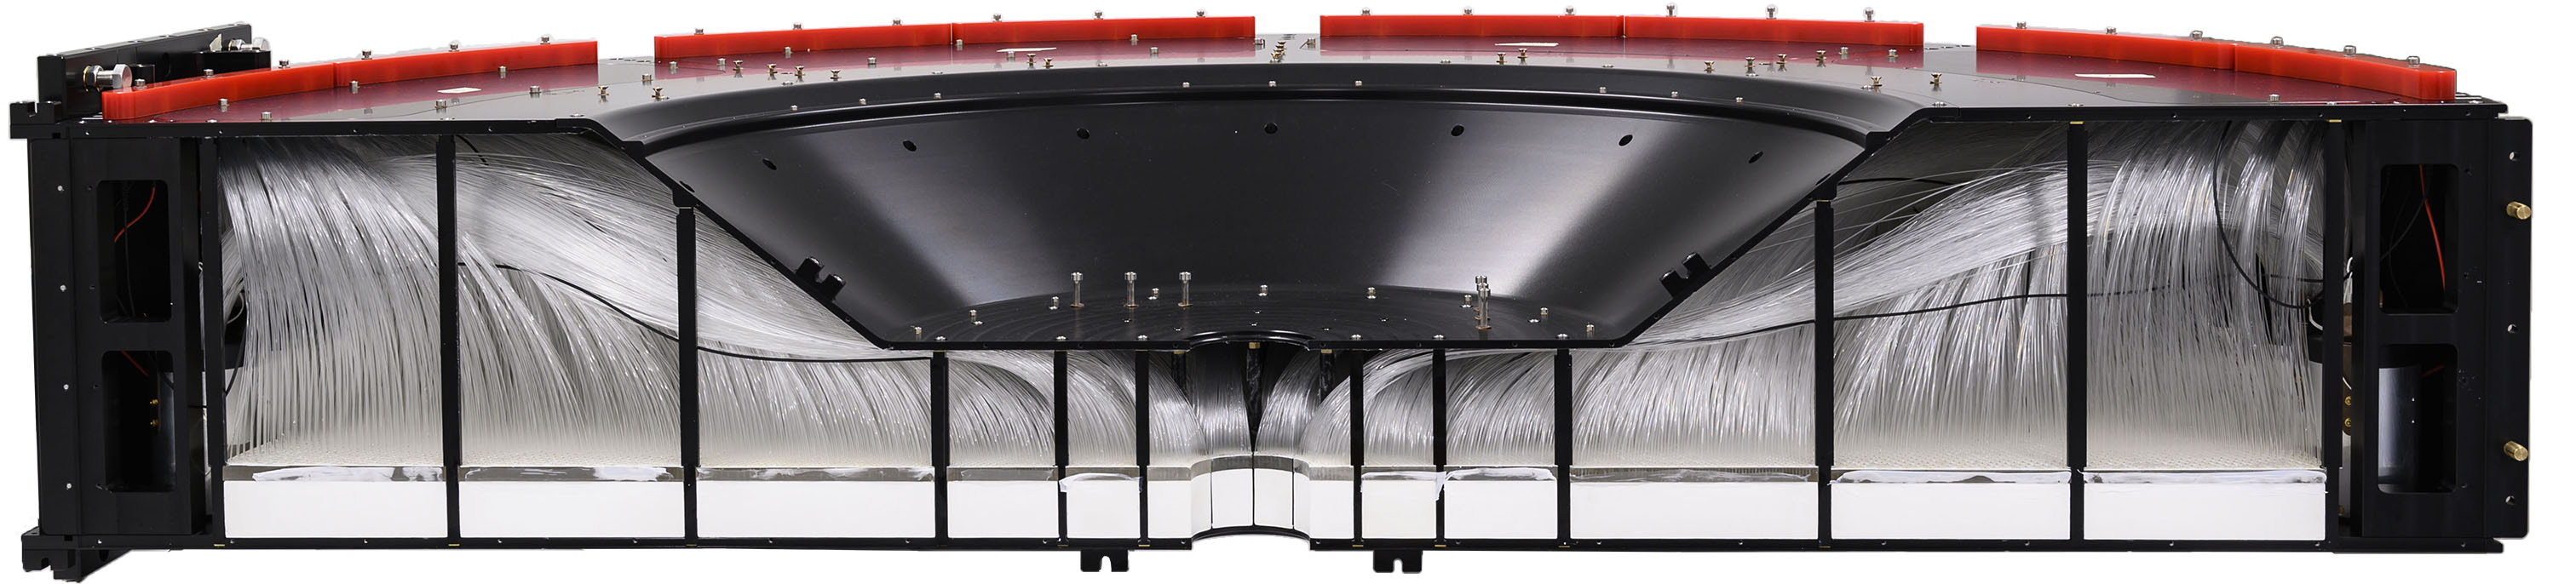
\includegraphics[width=0.9\linewidth]{fit/FV0_crossSection.jpg}
\caption{ Photograph of one half of the FV0. The optical fibers connect the scntillators to the PMTs on the rim of the support structure, the black structure seen here. The center wall has been removed to show the scintillator, surface matrix structure, and optical fibers.}
\label{FV0fig}
\end{center}
\end{figure}


\subsubsection{FDD}
The FDD \cite{Rojastorres} comprises  two nearly identical arrays, FDD-A and FDD-C, surrounding the beam pipe on opposite sides of the IP.  Each array consists of eight rectangular pads, $216 \times 181 \times 25\, \rm{mm}^3$ BC420 scintillator. The pads are assembled as  two overlapping layers of four sectors each. To make clearance for the beam pipe, a quadrant was removed from the innermost corner of each scintillator plate. The diameter of the removed quadrant on the FDD-A scintillators is 124 mm and 74 mm on the FDD-C as illustrated in fig.~\ref{FITschematic}. Each pad has two wavelengths shifting (WLS)
bars attached to the opposite sides of the scintillator. Clear optical fibres carry the light
from the WLS to H8409-70 PMTs. There are 8 independent FDD channels on each side of the IP.

Benefitting from the much improved ITS capability of heavy flavour tagging in the central barrel, the FDD contributes to the measurements of diffractive cross sections and studies of ultra-peripheral collisions. In pp collisions, the main physics objectives of the FDD are the studies of centrally produced exclusive states, measurements of cross sections for single and double diffraction, and inelastic processes at the new LHC centre of mass energy of 14 TeV. In Pb$-$Pb and p$-$Pb collisions, the FDD provides an independent measurement of centrality in an intermediate pseudorapidity range between the ITS and the ZDC and contributes to the selection of ultra-peripheral collisions. In the online mode, the FDD is used to monitor beam quality and to reject beam-gas events. 


\subsubsection{Electronics and readout scheme}

\begin{figure}[htbp]
\begin{center}
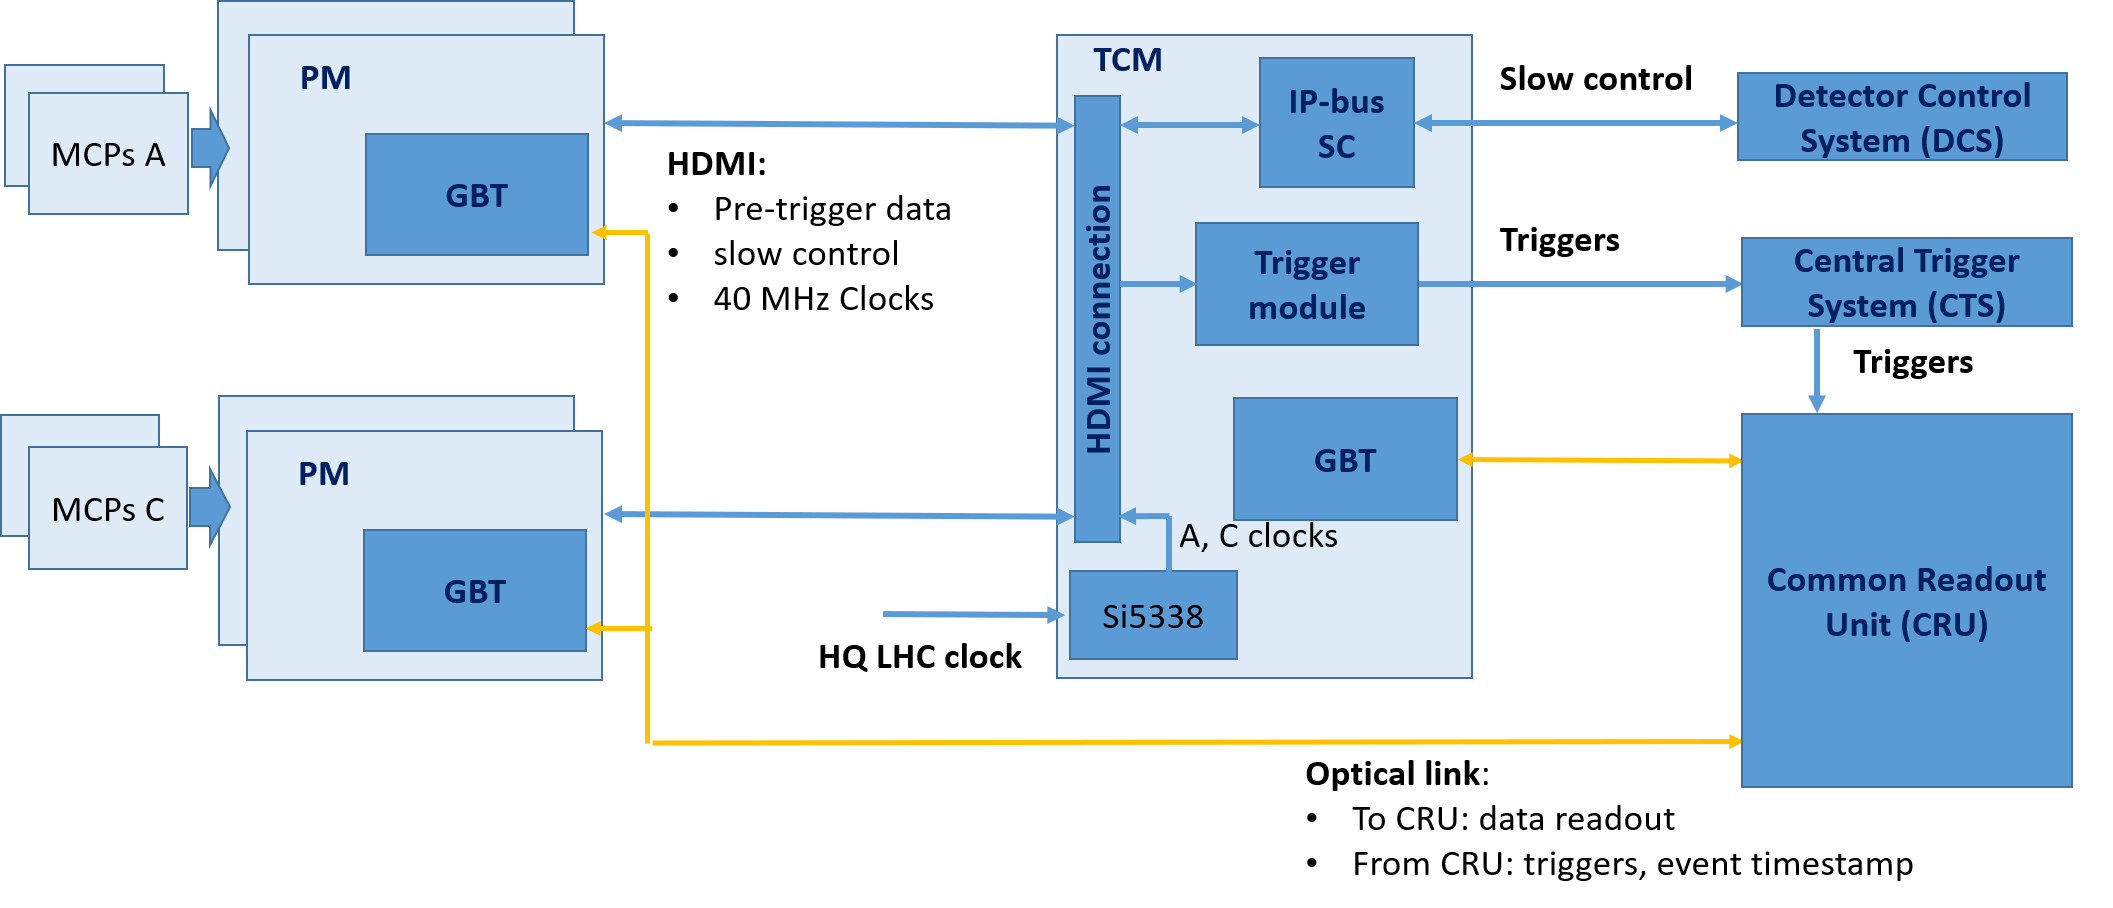
\includegraphics[width=0.9\linewidth]{fit/FIT_data_processing.png}
\caption{Schematic diagram of the FIT readout electronics. }
\label{default}
\end{center}
\end{figure}
All three subsystems of FIT use the same front-end and readout electronics based on just two custom-designed modules: a Processing Module (PM) and a Trigger and Clock Module (TCM). One PM provides 12 independent inputs. Each sub-detector has only one TCM while the number of PMs is determined by the number of channels. Each PM is connected to the dedicated TCM via an HDMI cable to transmit "pre-trigger" data, slow-control data and LHC clock distribution. The commands, configuration data, and status data are sent from the ALICE control system to the TCMs via a 1 Gb Ethernet optical link using an IPbus (UDP
based protocol) \cite{Finogeev:2020qkf}. The triggers and the measured event rates for the luminosity
measurements are transmitted from the TCMs via the same connection. The PMs are
configured from TCMs via an HDMI SPI connection. The PMs and TCMs are connected
to the ALICE DAQ with GBT links. FIT delivers the produced trigger signals to the Central Trigger System.
 
Laser pulses are used for time and amplitude calibration, as well as monitoring of ageing and radiation damage of the FIT detectors.

